\section {Aproximação da Equação de Helmholtz}

O método descrito na seção anterior mostra como podemos calcular a pressão acústica $\rho(u, t)$. Porém, desejamos na verdade calcular a Radiação Acústica gerada pela vibração do objeto. Nessa seção mostraremos como aproximamos a Radiação Acústica na nossa implementação.
Para cada ponto $u$ do domínio, desejamos calcular a Radiação Acústica $T(u) = A(u)e^{i\phi(u)}$. Consideremos, então, o sinal de um ponto fixo. Ao entrar em equilíbrio, o sinal $s(t)$ desse ponto poderá ser representado por $s(t) = A \cos(\omega t + \phi)$. Se calcularmos o valor médio\footnote{O valor médio $\mean{f}$ de uma função $f(t)$ é definido por $$\mean{f} = \frac{\int_a^b f(t)}{b-a}$$} $\mean{s}$ do valor absoluto sinal ao longo de um certo período, obteremos $\mean{|s|} = \frac{2A}{\pi}$. Logo, se soubermos $\mean{|s|}$ e $s(t)$ para um certo $t$, podemos calcular $A$ e $\phi$: 

\begin{equation}
	\begin{cases}
		A = \dfrac{\pi\mean{|s|}}{2}\\
		\phi = \arccos \left(\dfrac{s(t)}{A}\right) - \omega t
	\end{cases}
	\label{eq:amplitude_phase_estimation}
\end{equation}

Na nossa implementação, o valor médio do sinal de cada elemento do domínio é calculado utilizando uma \emph{Weighted Moving Average} (WMA), isto é:

\begin{equation}
	\mean{s}_{t} = \alpha\mean{s}_{t-1} + (1-\alpha)s(t)
\end{equation}

A amplitude $A$ e a fase $\phi$ são calculados a cada timestep utizando a fórmula \eqref{eq:amplitude_phase_estimation}. O valor médio de $A$ e $\phi$ também são calculados utilizando uma WMA. Em todos os casos, utilizamos $\alpha = 0.95$.

\subsection{Expansão Multipolar}

A nossa solução da equação da onda é calculada dentro de um domínio limitado. Não seria adequado limitar a síntese acústica para esse domínio. Já vimos, no entanto, que é possível calcular a transferência acústica para Far-Field utilizando a Integral de Kirchoff \eqref{kirchhorff_integral}.

Calcular a Integral de Kirchoff (uma integral de superfície) em tempo de execução é um procedimento custoso em termos de tempo e memória. Para evitar isso, exploramos a estrutura da Equação de Helmholtz.

A função de Green $G(u, v)$ da equação de Helmholtz pode ser decomposta numa base de funções \cite{gumerov2005fast}:

\begin{equation} \label{eq:helmholtz_expansion}
	G(u, v) = ik \sum_{n=0}^{\infty} \sum_{m=-n}^n S_n^m(u - u_0)R_n^{-m}(v - u_0)
\end{equation}

O ponto $u_0$ é o ponto no centro do Near-Field. A função $S_n^m$ é a Funcão Esférica Singular da Equação de Helmholtz e $R_n^m$ é a Funcão Esférica Singular da Equação de Helmholtz. Elas são definidas de acordo com as coordenadas polares $u = (r, \theta, \phi)$:

\begin{equation} \label{eq:helmholtz_basis_functions}
	\begin{cases}
		S_n^m(u) \Rightarrow S_n^m(r, \theta, \phi) = h_n^{(2)}(kr)Y_n^m(\theta, \phi)\\
		R_n^m(u) \Rightarrow R_n^m(r, \theta, \phi) = j_n(kr)Y_n^m(\theta, \phi)
	\end{cases}
\end{equation}

As funções $j_n : \mathbb{R}\rightarrow\mathbb{R}$ são as Funções Esféricas de Bessel. As funções $h_n^{(2)} : \mathbb{R}\rightarrow\mathbb{C}$ são a Funções Esféricas de Hankell de segunda espécie. As funções $Y_n^m : \mathbb{R}\times\mathbb{R}\rightarrow\mathbb{C}$ são os Harmônicos Esféricos (Ver \figref{fig:spherical_harmonics}). Essas funções aparecem constantemente em diversos ramos da ciência\footnote{O uso de Funções Esféricas é comum em ramos como Eletromagnetismo, Mecânica Quântica, Acústica e Computação Gráfica.} por elas formam uma base para o espaço de funções em $\mathbb{R}^3 \rightarrow \mathbb{R}$. A sua estrutura permite explorar a simetria radial e também permite aproximar funções com apenas alguns termos.

\begin{figure}[ht]
	\centering
	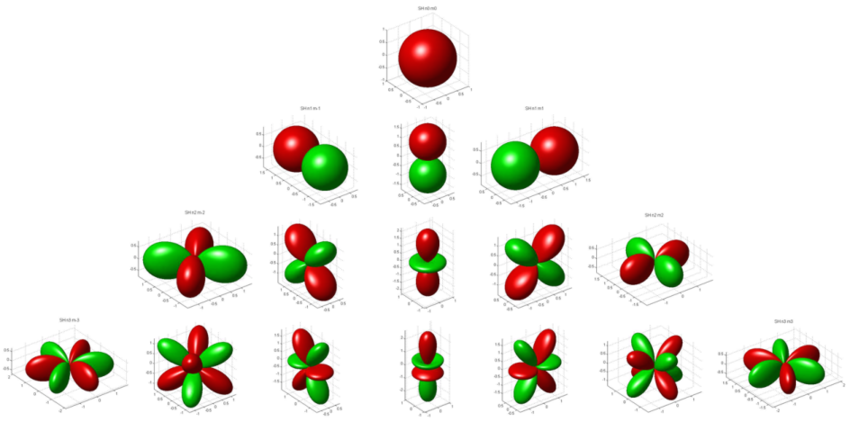
\includegraphics[width=\textwidth]{algorithm/spherical_harmonics.png}
	\caption[Harmônicos Esféricos]{Harmônicos Esféricos}
	\label{fig:spherical_harmonics}
\end{figure}

Se aplicarmos a expansão da Função de Green \eqref{eq:helmholtz_expansion} na Integral de Kirchoff \eqref{kirchhorff_integral}, obteremos:

\begin{equation}\label{eq:multipole_expansion}
\begin{split}
	T(u) =& \int_{\Gamma} \left[G(u, v)\frac{\partial T}{\partial n}(v) - \frac{\partial G}{\partial n}(u, v)T(v) \right] d\Gamma_v\\
	% 
	=& \int_{\Gamma} \left[ik \sum_{n=0}^{\infty} \sum_{m=-n}^n S_n^m(u - u_0)R_n^{-m}(v - u_0)\frac{\partial T}{\partial n}(v)\right.\\
	&\quad\left. - ik \sum_{n=0}^{\infty} \sum_{m=-n}^n S_n^m(u - u_0)\frac{\partial R_n^{-m}}{\partial n}(v - u_0)T(v) \right] d\Gamma_v\\
	% 
	=& \sum_{n=0}^{\infty} \sum_{m=-n}^n S_n^m(u - u_0)ik \int_{\Gamma}\left[ R_n^{-m}(v - u_0)\frac{\partial T}{\partial n}(v) -  \frac{\partial R_n^{-m}}{\partial n}(v - u_0)T(v)\right]d\Gamma_v\\
	%
	=& \sum_{n=0}^{\infty} \sum_{m=-n}^n S_n^m(u - u_0)M_n^m
\end{split}
\end{equation}

Os termos $M_n^m$ são chamados de \emph{Coeficientes Multipolares}. Eles podem ser precomputados utilizando a fórmula:

\begin{equation}
	M_n^m = ik \int_{\Gamma}\left[ R_n^{-m}(v - u_0)\frac{\partial T}{\partial n}(v) -  \frac{\partial R_n^{-m}}{\partial n}(v - u_0)T(v)\right]d\Gamma_v
\end{equation}

Esses termos podem ser utilizados para calcular a Radiação Acústica $T(u)$ em tempo de execução utilizando a fórmula \eqref{eq:multipole_expansion}. Na nossa implementação, os coeficientes são calculados em paralelo na GPU. Nós utilizamos as recursões apresentada em \cite{press2007numerical} para calcular a Funções Esféricas. A \figref{fig:multipole_comparison} apresenta uma comparação entre o valor calculado da Radiação Acústica e o valor aproximado com a Expansão Multipolar.  


\begin{figure}[ht]
\centering
\begin{subfigure}{0.5\textwidth}
	\centering
	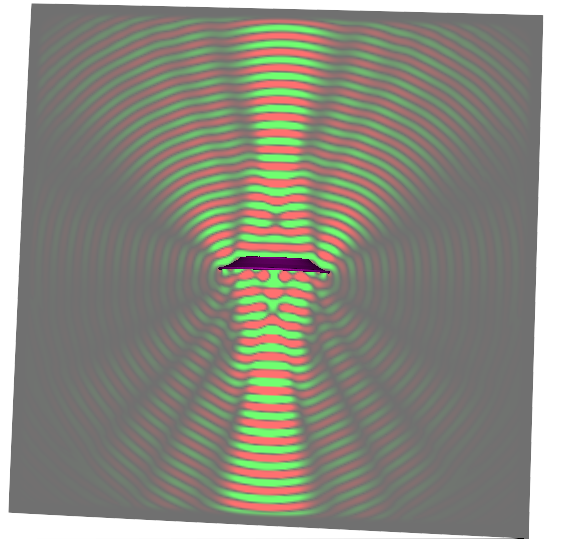
\includegraphics[width=\textwidth]{algorithm/plate_mode_a.png}
	\caption{Ground Truth}\label{fig:acoustic_transfer_ground_truth}
\end{subfigure}%
\begin{subfigure}{0.5\textwidth}
	\centering
	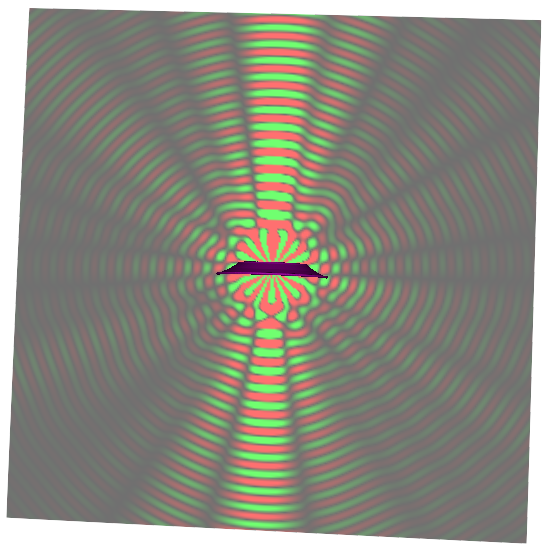
\includegraphics[width=\textwidth]{algorithm/plate_mode_b.png}
	\caption{Aproximação Multipolar com $\bar{n} = 16$}
	\label{fig:acoustic_transfer_multipole_estimate}
\end{subfigure}
\caption[Comparação entre o Ground Truth da Radiação Acústica e a aproximação Expansão Multipolar]{Comparação entre o Ground Truth da Radiação Acústica e a aproximação Expansão Multipolar. O objeto é um Prato de Cerâmica oscilando no Modo 23 a 10215.97Hz}
\label{fig:multipole_comparison}
\end{figure}